You've been put in charge of an art exhibit from the famous minimalist sculptor J (even his name is minimalist!). 
J's work involves the careful layout of vertically dispositioned orthogonal parallelpipeds in a set of tapering 
obelisks -- in other words, he puts smaller boxes on top of larger boxes. 
His most recent triumph is called ``2 by 3's Decreasing,'' in which he has various sets of six boxes arranged in 
two stacks of three boxes each. One such set is shown below:

\begin{figure}[h]
\center
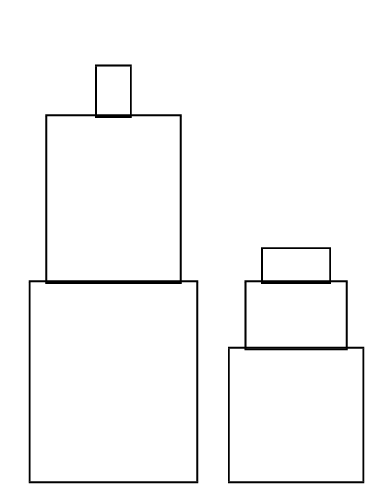
\includegraphics[width=0.20\textwidth ]{image/A.png}
\end{figure}

J has sent you the art exhibit and it is your job to set up each of the six-box sets at various locations 
throughout the museum. But when the sculptures arrived at the museum, uncultured barbarians (i.e., delivery men) 
simply dropped each set of six boxes on the floor, not realizing the aesthetic appeal of their original layout. 
You need to reconstruct each set of two towers, but you have no idea which box goes on top of the other! 
All you know is the following: for each set of six, you have the heights of the two towers, 
and you know that in any tower the largest height box is always on the bottom and the smallest 
height box is on the top. Armed with this information, you hope to be able to figure out which 
boxes go together before tomorrow night's grand opening gala.
